\documentclass[8pt,landscape,a4paper]{article}
\usepackage[utf8]{inputenc}
\usepackage[ngerman]{babel}
\usepackage[T1]{fontenc}
%\usepackage[LY1,T1]{fontenc}
%\usepackage{frutigernext}
%\usepackage[lf,minionint]{MinionPro}
\usepackage{tikz}
\usetikzlibrary{shapes,positioning,arrows,fit,calc,graphs,graphs.standard}
\usepackage[nosf]{kpfonts}
\usepackage[t1]{sourcesanspro}
\usepackage{multicol}
\usepackage{wrapfig}
\usepackage[top=0mm,bottom=1mm,left=0mm,right=1mm]{geometry}
\usepackage[framemethod=tikz]{mdframed}
\usepackage{microtype}
\usepackage{pdfpages}
\usepackage{graphicx}
\usepackage{lipsum}  % generates filler text
\usepackage{xcolor}
\usepackage{listings}
\usepackage{xparse}
\usepackage{courier} %% Sets font for listing as Courier.


\let\bar\overline

\definecolor{myblue}{cmyk}{1,.72,0,.38}
\definecolor{orange}{rgb}{1,0.5,0}
\definecolor{mynicegreen}{RGB}{5,255,102}

\def\firstcircle{(0,0) circle (1.5cm)}
\def\secondcircle{(0:2cm) circle (1.5cm)}

\colorlet{circle edge}{myblue}
\colorlet{circle area}{myblue!5}

\tikzset{filled/.style={fill=circle area, draw=circle edge, thick},
    outline/.style={draw=circle edge, thick}}
    
\pgfdeclarelayer{background}
\pgfsetlayers{background,main}

\everymath\expandafter{\the\everymath \color{myblue}}
\everydisplay\expandafter{\the\everydisplay \color{myblue}}

\renewcommand{\baselinestretch}{.8}
\pagestyle{empty}

% \global\mdfdefinestyle{header}{%
% linecolor=gray,linewidth=1pt,%
% leftmargin=0mm,rightmargin=0mm,skipbelow=0mm,skipabove=0mm,
% }

% \newcommand{\header}{
% \begin{mdframed}[style=header]
% \footnotesize
% \sffamily
% Hilfszettel zur Klausur\\
% von~Jigao,~Seite~\thepage~von~2
% \end{mdframed}
% }

\makeatletter % Author: https://tex.stackexchange.com/questions/218587/how-to-set-one-header-for-each-page-using-multicols
\renewcommand{\section}{\@startsection{section}{1}{0mm}%
                                {0ex}%
                                {.1ex}%x
                                {\color{myblue}\sffamily\small\bfseries}}
% \renewcommand{\subsection}{\@startsection{subsection}{1}{0mm}%
%                                 {0ex}%
%                                 {.1ex}%x
%                                 {\color{myblue}\sffamily\bfseries}}
\newcommand{\rtext}[1]{\textcolor{red}{\textbf{#1}}}
\newcommand{\redtext}[1]{\textcolor{red}{#1}}
\newcommand{\btext}[1]{\textcolor{blue}{\textbf{#1}}}
\newcommand{\bluetext}[1]{\textcolor{blue}{#1}}
\newcommand{\orangetext}[1]{\textcolor{orange}{#1}}
\newcommand{\greentext}[1]{\textcolor{mynicegreen}{#1}}
\newcommand{\mysubsection}[1]{\textcolor{myblue}{\scriptsize{\textbf{#1}}}}
\newcommand{\hlc}[2][yellow]{{%
    \colorlet{foo}{#1}%
    \sethlcolor{foo}\hl{#2}}%
}
\newcommand{\hlgray}[1]{%
  \hlc[lightgray!40]{#1}
}

% \def\multi@column@out{%
%    \ifnum\outputpenalty <-\@M
%    \speci@ls \else
%    \ifvoid\colbreak@box\else
%      \mult@info\@ne{Re-adding forced
%                break(s) for splitting}%
%      \setbox\@cclv\vbox{%
%         \unvbox\colbreak@box
%         \penalty-\@Mv\unvbox\@cclv}%
%    \fi
%    \splittopskip\topskip
%    \splitmaxdepth\maxdepth
%    \dimen@\@colroom
%    \divide\skip\footins\col@number
%    \ifvoid\footins \else
%       \leave@mult@footins
%    \fi
%    \let\ifshr@kingsaved\ifshr@king
%    \ifvbox \@kludgeins
%      \advance \dimen@ -\ht\@kludgeins
%      \ifdim \wd\@kludgeins>\z@
%         \shr@nkingtrue
%      \fi
%    \fi
%    \process@cols\mult@gfirstbox{%
% %%%%% START CHANGE
% \ifnum
% \count@=\numexpr\mult@rightbox+2\relax
%           \setbox\count@\vsplit\@cclv to \dimexpr \dimen@-1cm\relax
% % \setbox\count@\vbox to \dimen@{\vbox to 1cm{\header}\unvbox\count@\vss}%
% \else
%       \setbox\count@\vsplit\@cclv to \dimen@
% \fi
% %%%%% END CHANGE
%             \set@keptmarks
%             \setbox\count@
%                  \vbox to\dimen@
%                   {\unvbox\count@
%                    \remove@discardable@items
%                    \ifshr@nking\vfill\fi}%
%            }%
%    \setbox\mult@rightbox
%        \vsplit\@cclv to\dimen@
%    \set@keptmarks
%    \setbox\mult@rightbox\vbox to\dimen@
%           {\unvbox\mult@rightbox
%            \remove@discardable@items
%            \ifshr@nking\vfill\fi}%
%    \let\ifshr@king\ifshr@kingsaved
%    \ifvoid\@cclv \else
%        \unvbox\@cclv
%        \ifnum\outputpenalty=\@M
%        \else
%           \penalty\outputpenalty
%        \fi
%        \ifvoid\footins\else
%          \PackageWarning{multicol}%
%           {I moved some lines to
%            the next page.\MessageBreak
%            Footnotes on page
%            \thepage\space might be wrong}%
%        \fi
%        \ifnum \c@tracingmulticols>\thr@@
%                     \hrule\allowbreak \fi
%    \fi
%    \ifx\@empty\kept@firstmark
%       \let\firstmark\kept@topmark
%       \let\botmark\kept@topmark
%    \else
%       \let\firstmark\kept@firstmark
%       \let\botmark\kept@botmark
%    \fi
%    \let\topmark\kept@topmark
%    \mult@info\tw@
%         {Use kept top mark:\MessageBreak
%           \meaning\kept@topmark
%          \MessageBreak
%          Use kept first mark:\MessageBreak
%           \meaning\kept@firstmark
%         \MessageBreak
%          Use kept bot mark:\MessageBreak
%           \meaning\kept@botmark
%         \MessageBreak
%          Produce first mark:\MessageBreak
%           \meaning\firstmark
%         \MessageBreak
%         Produce bot mark:\MessageBreak
%           \meaning\botmark
%          \@gobbletwo}%
%    \setbox\@cclv\vbox{\unvbox\partial@page
%                       \page@sofar}%
%    \@makecol\@outputpage
%      \global\let\kept@topmark\botmark
%      \global\let\kept@firstmark\@empty
%      \global\let\kept@botmark\@empty
%      \mult@info\tw@
%         {(Re)Init top mark:\MessageBreak
%          \meaning\kept@topmark
%          \@gobbletwo}%
%    \global\@colroom\@colht
%    \global \@mparbottom \z@
%    \process@deferreds
%    \@whilesw\if@fcolmade\fi{\@outputpage
%       \global\@colroom\@colht
%       \process@deferreds}%
%    \mult@info\@ne
%      {Colroom:\MessageBreak
%       \the\@colht\space
%               after float space removed
%               = \the\@colroom \@gobble}%
%     \set@mult@vsize \global
%   \fi}

\makeatother
\setlength{\parindent}{0pt}

\NewDocumentCommand{\codeword}{v}{%
\texttt{\textcolor{blue}{#1}}%
}

% \lstset{language=Java, breakatwhitespace=true, keywordstyle={\bfseries \color{blue}}}

\lstset{
  language=Java,
  tabsize = 2, %% Sets tab space width.
  showstringspaces = false, %% Prevents space marking in strings, string is defined as the text that is generally printed directly to the console.
  numbers = left, %% Displays line numbers on the left.
  commentstyle = {\bfseries \color{green}}, %% Sets comment color.
  keywordstyle = {\bfseries \color{blue}}, %% Sets  keyword color.
  stringstyle = {\bfseries \color{red}}, %% Sets  string color.
  rulecolor = {\bfseries \color{black}}, %% Sets frame color to avoid being affected by text color.
  basicstyle = \small \ttfamily , %% Sets listing font and size.
  breaklines = true, %% Enables line breaking.
  numberstyle = \tiny,
}

\begin{document}
%\footnotesize
\small
\begin{multicols*}{5}
\section{Introduction}
\redtext{Enterprise SY architecture:}Cs, Web S, APP Ss, MsgQueue, Pub/Sub SY, DBs 
\\ 
\redtext{Distributed APP} developed on \bluetext{sockets}.
(Fallacies,
Interoperability in spite of heterogeneity,
Data representation and encoding,
Parameter passing convention calling remote procedures,
Atomic execution of TX,
Enable APP integration,
Data persistence)
\\
\redtext{Middleware} as layer between \bluetext{transport \& application layer}
or \bluetext{Above OS and below APP}. 
comprises \bluetext{services and abstractions}(RMI, Messaging, PubSub,TX,Naming) that facilitate the
design, development, and deployment of distributed APP in
\bluetext{heterogeneous, networked environments}.
Deals with interoperability
\begin{CJK*}{UTF8}{gbsn}
\bluetext{互通性}
\end{CJK*}, SY integration
\textbar 
C request/response $\leftrightarrow$ Middleware $\leftrightarrow$ S. 
\textbar
All Computers \bluetext{share single distributed APP and Middleware.}
\\
\redtext{Heterogeneity}:
Computer architecture(big, little endian), 
OS(Comm. sub-system), 
Host and network representation of data, 
Programming language(Representation of characters)
\\
\redtext{Ilities:}
Reliable; 
Fault-tolerant; 
Highly available; 
Recoverable; 
Consistent; 
Scalable; 
Predictable pref.; 
Secure; 
Heterogeneous; 
Open
% \\
% \rtext{8 Fallacies}
% \rtext{1.Network Reliable} 
% \bluetext{Assumptions:}Power Supply, Hard Disk, Node Failures, Config., Bugs
% \bluetext{Effect:}APP hangs, crashes 
% \bluetext{Countermeasures:}
% Redundancy HW\&SW systems,middleware \&application; 
% Catch Exceptions; 
% Check Codes, React; 
% Retry After Timeouts;
% pos. neg. ACK; 
% Identify \& ignore duplicates; 
% idempotent operations
% \rtext{2.Latency\begin{CJK*}{UTF8}{gbsn}延迟\end{CJK*} Is Zero}
% time For Data Transfer(speed Of Light); 
% Bandwidth:how Much Data transferred (bit/s)
% \textbar
% Local Call: Push and a Jump to Subroutine;
% SY Call: OS, 100s of assembly;
% Call across LAN: SY calls on caller $+$ callee $+$ network latency;
% Call across WAN: transmission delay
% \redtext{3.Bandwidth is infinite.
% 4.The network is secure.
% 5.Topology doesn't change.
% 6.There is one administrator.
% 7.Transport cost is zero.
% 8.The network is homogeneous}
% \\
% \bluetext{Standardization}:
% Official:ISO, ITU, DIN, Semi-official: IEEE, W3C, OpenGroup
\section{Comm. Basics}
\redtext{ISO OSI:}
Open Systems Interconnection model, 
Basis for standards development on SY interconnection,
Reference model.
\textbar
\redtext{Layers:}
\bluetext{
Application(Peer protocol: HTTP, DNS, FTP);
Presentation;
Session;
Transport: TCP/UDP;
Network: IP;
Data link;
Physical}
\\ 
\redtext{IPv4 v6(no checksum):}
Relays datagrams accross networks,
Routing enables internetworking,
Deliver packet from source to host address,
Foundation for TCP/UDP
\\
\redtext{IP routing:}routing protocol,
\bluetext{BGP} used in internet:
Border Gateway Protocol,
Routing between AS (Autonomous systems, provider or bigger organization),
Exchanges routing and reachability information between AS.
\\
\redtext{TCP:} for \bluetext{HTTP, RPC},
Slower than UDP, but with reliability using ACK,
Connection oriented protocol, session is initiated,
Provides ordering, sequencing,
Flow control, sender can't overflow receiver(same speed sending, receiving),
PortNum in TCP protocol(not in IP protocol)
\\
\redtext{UDP:} for \bluetext{DNS, Video, Voice},
Faster than TCP,
Connectionless(no session);
Best-effort;
Packet independent; 
No guaranteed delivery;
No ordering guarantees;
P2P and P2-multipoint.
\\
\redtext{Ports:}
a 16 bit number to local host to identify the connection, 
to differentiate APPs, if packet arrive;
Separate for \bluetext{UDP and TCP};
$0-1023$ reserved to root,
$1024 - 65535$  available to regular user;
http 80/tcp, ftp 21/tcp, ssh 22/tcp, telnet 23/tcp, finger 79/tcp, snmp 161/udp
\\
\redtext{APP Layer protocol:}
Set of rules specifying data transfer
between computing end-points
(Connection establishment \& tear-down
Data representation,
Comm);
\bluetext{DHCP} (Dynamic Host Configuration Protocol),
\bluetext{HTTP} (Hypertext Transfer Protocol),
\bluetext{FTP} (File Transfer Protocol),
\bluetext{Telnet} (Telnet Remote Protocol),
\bluetext{SSH} (Secure Shell Remote Protocol),
\bluetext{SIP} (Session Initiation Protocol),
\bluetext{POP3} (Post Office Protocol 3),
\bluetext{SMTP} (Simple Mail Transfer Protocol),
\bluetext{IMAP} (Internet Message Access Protocol),
\textbar \textbar
browser retreives web page(HTTP 1.1 over TCP, HTTP, FTP, SMTP)
\\
\redtext{HTTP/1.0 C S:}
\bluetext{Request}: GET <path>/index.html HTTP/1.0
\bluetext{Response}: HTTP/1.0 200 OK
\bluetext{ErrorResponse}: HTTP/1.0 404 Not Found 
\textbar \textbar
\redtext{HTTP/1.1:}
HyperText Transfer Protocol,
Request/Response protocol for C S comm. on top of TCP
(Browser,
RESTFUL API‘s,
SOAP over HTTP,
NoSQL databases)
\bluetext{Methods:}
\bluetext{GET:}cacheable get info by Request-URI
\bluetext{HEAD:} like GET but MUST NOT return a message-body
\bluetext{POST:} post a form (bulletin board), uploading data,
can be a data-accepting process
Responses not cacheable(200 (OK), 204(No Content), 201
(Created), 303 (See Other)) 
\bluetext{PUT:} Enclosed entity to be stored under Request-URI
Responses not cacheable
\bluetext{DELETE:} Delete the resource by Request-URI
Response: 200 (OK), 202 (Accepted), 204 (No Content)
\bluetext{TRACE:} for diagnostics
\bluetext{CONNECT:} to initialize secure connection, HTTPS on port 443,
Proxy is asked to forward the TCP connection
\textbar
\redtext{HTTP/1.1 proxy:}C \bluetext{GET req.} $\rightarrow$ Proxy, but not in cache. 
Proxy \bluetext{GET req.} $\rightarrow$ Origin, Origin $\rightarrow$ Proxy response.
C \bluetext{GET req.} $\rightarrow$ Proxy, Proxy $\rightarrow$ C cached resp.
\textbar
\redtext{HTTP/2.0:}
Better utilization network capacity,
Headers compressed,
On a single connection req and resp interleaved,
Prioritization of requests
% FIXME: can be removed
\textbar \textbar \textbar
GET/HTTP/1.1
Host:www.tum.de
Connection:keep-alive
Accept: text/html,application/xhtml+xml,application/xml;q=0.9, image/webp, */*;q=0.8
User-Agent: Mozilla/5.0 (X11; Linux x86\_64) AppleWebKit/537.36 (KHTML, like Gecko) Chrome/37.0.2062.120 Safari/537.36
Accept-Encoding: gzip,deflate,sdch
\textbar \textbar \textbar
HTTP/1.1 200 OK
Date: Wed, 08 Oct 2014 15:25:53 GMT
Server: Apache
X-Powered-By: PHP/5.5.17
Content-Encoding: gzip
%
%
%
\\
\mysubsection{Socket}
\\
Move data/Msg/(invoke operation/service and return result/failure) 
from APP I on Host A to APP K on Host B.
\redtext{Client}:Issues req to S(send \& receive).
\redtext{Server}:Starts up and listens for connections, req.s, and sends/receives.
\redtext{C S eg.}: \bluetext{P2P} telnet/telnetd, ftp/ftpd (sftp/sftpd), Firefox/Apache.
\\
\rtext{Socket}: using network API, network programming abstraction for comm. among processes (APPs) based on (Unix) file
descriptors.
\bluetext{File/Socket descriptor}:int for open file managed by the OS, 
In \orangetext{Unix any I/O} by reading/writing from/to file descriptors.
\textbar
\redtext{Socket types}: 
\bluetext{Stream socket:}telent, HTTP, browser, java.net.ServerSocket, TCP based(Ordering guaranteed, Error-free); 
\bluetext{Datagram socket:}java.net.DatagramSocket, UDP based; 
\bluetext{IPv4\&IPv6}
\\
\redtext{2 end-points determine a connection}: IP address (host address)$+$Port number
\\
\rtext{SetUp,UseSockets}
\orangetext{S Create:}
\lstinline{final ServerSocket ss = new;/*localhost only*/ ss.bind(new InetSocketAddress("0.0.0.0", port)); while (true) {Socket clientSocket = ss.accept();/*Block till C*/}
\orangetext{C connect S:}
\lstinline{Socket s = new; s.connect(new InetSocketAddress("127.0.0.1", port)); PrintWriter output = new PW(s.getOutputStream()); BufferedReader input = new BR(new InputStreamReader(s.getInputStream())); output.write(req + "\r\n");/*to S*/ output.flush();}
\orangetext{S handle req.:}
\lstinline{/*in while true*/ BufferedReader in = new BR(new InputStreamReader(clientSocket.getInputStream(), Constants.TELNET_ENCODING)); PrintWriter out = new PW(new OutputStreamWriter(clientSocket.getOutputStream(), Constants.TELNET_ENCODING)); String firstLine; while ((firstLine = in.readLine()) != null) /*req from C*/ String res = kv.process(firstLine); out.write(res); /*to C*/ out.flush();}
\orangetext{C read resp.:}
\lstinline{/*after C connect S*/String response = input.readline(); s.close();}
\orangetext{S shutdown:}
\lstinline{ss.close();}
\adjincludegraphics[width=1\linewidth, trim={0 0 0 {.12\height}},clip]{chap1_1.png}
\redtext{\hlgray{Finite state machines FSM}} \hlgray{describing} 
\redtext{\hlgray{a comm. session C S}}.
\hlgray{C\&S keep comm. session open and exchange Msg until one of them closed.}
\orangetext{\hlgray{accept:}} \hlgray{a} \lstinline{while loop}:
\orangetext{\hlgray{create a new socket (and th.) for commu. with C}}
\\
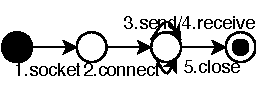
\includegraphics[width=.49\linewidth]{client_FSM.pdf}
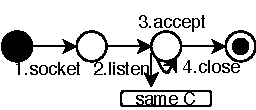
\includegraphics[width=.49\linewidth]{server_FSM.pdf}
\rtext{K V Server:} C get, set Table in S: 
\bluetext{PUT tablename key value\textbackslash r\textbackslash n}, 
\bluetext{GET tablename key}
\textbar
\redtext{C:}
\orangetext{C.java:}
\lstinline{KVTable<AssessmentInformation> kvc = new KVTable<~>(); kvc.put("middleware", new AssessmentInformation(1.3);}
\orangetext{KVTable.java in put():}
\lstinline{String jsonStr = gs.toJson(value); String enc_value = encodeBase64(jsonStr); this.activeConnection.write("PUT " + this.table + " " + key + " " + enc_value + "\r\n");}
\orangetext{ActiveConnection.java in write():}
\lstinline{PrintWriter output...; output.write(..); output.flush();}
\redtext{S:}
\orangetext{ConnectionHandleThread.java}
\lstinline{BufferedReader in = new BufferedReader(new ISReader(clientSocket.getIS(),...)); String line = in.readLine();}
\orangetext{KVStore.java}
\lstinline{StringTokenizer st = new StringTokenizer(firstLine, " \r\n"); String command = st.nextToken(); if (command == "GET")/*GET PUT else*/}
\orangetext{ConnectionHandleThread.java}
\lstinline{PrintWriter out = new PrintWriter(new OutputStreamWriter(clientSocket.getOutputStream(),...)); out.write(res);/*to C*/ out.flush();}
\\
\mysubsection{NIO(NonblockingSockets),multi.threaded}
\\
\redtext{Synchronous}: 
Single th. read data from C(stream) and blocked until done
\rtext{Asynchronous}: 
th. $\rightarrow$ \bluetext{Channel}: 
read data into \bluetext{Buffer}; 
\bluetext{Channel} $\rightarrow$ \bluetext{Buffer}: 
fill data into \bluetext{Buffer}; 
Th. $\rightarrow$ \bluetext{Buffer}: 
check data in \bluetext{Buffer} (main th. not blocked)
\\
\rtext{\hlgray{Syn. vs. Asyn.}}: 
\bluetext{Syn}: Th. acts and waits until \orangetext{Syn. I/O} done; 
\orangetext{}text{Limited scalability}, a th. per I/O connection
(Overhead:\orangetext{context switching} $\rightarrow$ time between diff. tasks)
\bluetext{Asyn}: Pass req. to OS-kernel and do other tasks 
$\rightarrow$\orangetext{worker th.}\lstinline{while(true)} 
\rtext{++:}
\orangetext{\hlgray{only Compute, never Blocked, no Context Swtich, Asyn. I/O}}
\hlgray{
Scalability, 
Consumers not block S long time,
One th. handle multi. sockets
}
\rtext{--:}
\hlgray{
Complex handling code,
Requires different kind of architecture(Eventloops)
}
\\
\rtext{Java NIO Channels}: 
All \orangetext{I/O operations} done with \bluetext{channels(File, TCP, UDP)};
Multi types of \bluetext{channels}
(FileChannel(File on disk), 
DatagramChannel (UDP), 
SocketChannel (TCP, support concurrent read/write), 
ServerSocketChannel (TCP));
Responsibility(\orangetext{Read, write buffer})
\\
\rtext{\hlgray{Sequence Dia multi th:}}
\btext{\hlgray{n times C and Th.}}
\textbar
\bluetext{\hlgray{Ci to S:}} \hlgray{connect}, 
\bluetext{\hlgray{S to Th.i}}, 
\bluetext{\hlgray{Ci to S to Th.i:}} \hlgray{getTime()},
\bluetext{\hlgray{Th.i to S to C:}} \hlgray{20:00}
\\
\rtext{\hlgray{S Create:}} 
\hlgray{same as single th. above}
\orangetext{\hlgray{S Create}}
\bluetext{\hlgray{instead of block IO in while:}}
\lstinline{HandleRequest hr = new HandleRequest(client); hr.start();}
\\
\rtext{\hlgray{HandleRequest as Th.:}}
\lstinline{class HandleRequest extends Thread{private Socket c;HandleRequest(Socket c){c = c;/*]*/run(){String msg = c.receive()if(msg == "getTime"){String res = getTime();c.send(res);c.close();}
\\
\rtext{\hlgray{C:}}
\lstinline{class Client{public void sendMessage(){String ip'112.32.86.113'; int port = 8883; String msg = "getTime"; Socket c = new Socket(); c.connect(ip, port); c.send(msg); String res = client.receive(); client.close(); print res;}
\\
\rtext{\hlgray{Sequence Dia single th:}}
\btext{\hlgray{n times C}}
\textbar
\bluetext{\hlgray{Ci to S:}} \hlgray{connect}, 
\bluetext{\hlgray{Ci to S to Th.i:}} \hlgray{getTime()},
\hlgray{all C sent, S start with Zeitraum to process n req.}
\bluetext{\hlgray{Th.i to S to C:}} \hlgray{20:00 resp. same order as sent req.}
\\
\redtext{\hlgray{Selector:}} 
\hlgray{select multi asyn. Channels to match a EventLoop}
\orangetext{\hlgray{Setup channel:}}
\lstinline{Hashmap<SocketChannel, byte[]> pendingData; ServerSocketChannel ssc = new SSC(); ssc.connect("127.0.0.1", 8883); Selector selector = new Selector(); ssc.register(selector, SelectionKey.ACCEPT);}
\rtext{OR}
\lstinline{ServerSocketChannel ssC = SSC.open();ssC.configureBlocking(false);InetSocketAddress isa  = new ISA(InetAddress.getByName("localhost"), 5559);ssC.socket().bind(isa);}
\orangetext{\hlgray{handleRequest():}}
\lstinline{public byte[] handleRequest(byte[] input){return Bytes.toBytes(System.nanoTime());}
\orangetext{\hlgray{Eventloop:}}
\lstinline{public void start() throws IOException {while (true) try {selector.select();/*get List*/ Iterator selectedKeys = selector.selectedKeys().iterator(); while (selectedKeys.hasNext()) {SelectionKey key = (SelectionKey) selectedKeys.next(); selectedKeys.remove(); if (key.isAcceptable()) {ServerSocketChannel channel = (SSC)key.channel(); SocketChannel sC = channel.accept(); sC.configureBlocking(false); sC.register(this.selector, SelectionKey.READ);/*wake up when sth to read*/ else if (key.isReadable()) {SocketChannel channel = (SC)key.channel(); byte[] res = handleRequest(channel.read()); pendingData.add(channel, res); key.interesOps(SelectionKey.WRITE); else if (key.isWritable()) {SocketChannel channel = (SC)key.channel(); data = pendingData.get(channel); if(data == (byte[])"getTime"){channel.write((byte[])getTime()); key.interestOps(SelectionKey.READ); catch (e) {e.printStackTrace();}
% \orangetext{Register selector:}
% \lstinline{Selector s = SelectorProvider.provider().openSelector(); serverChannel.register(s, SelectionKey.OP_ACCEPT); private void accept(SelectionKey key) throws IOException {ServerSocketChannel sSC = (SSC) key.channel(); SocketChannel sC = sSC.accept(); sC.configureBlocking(false); sC.register(this.s, SelectionKey.OP_READ);/*wake up when sth to read*/}
\orangetext{Read:}
\lstinline{private void read(SelectionKey key) throws IOException {SocketChannel sC = (SC) key.channel(); this.readBuffer.clear(); int numRead = sC.read(this.readBuffer);/*in Buffer*/ if (numRead == -1) { key.channel().close(); key.cancel(); return;/*]*/byte[] dataCopy = new byte[numRead]; arraycopy(this.readBuffer.array(), 0, dataCopy, 0, numRead); handleRequest(sC, dataCopy);}
\orangetext{Write:}
\lstinline{private void write(SelectionKey key) throws IOException { SocketChannel sC = (SC) key.channel(); List queue = (List) this.pendingData.get(sC); while (!queue.isEmpty()) { ByteBuffer buf = (ByteBuffer) queue.get(0); socketChannel.write(buf); if (buf.remaining() > 0) {break;/*]*/queue.remove(0);/*]*/ if (queue.isEmpty()) {key.interestOps(SelectionKey.OP\_READ);/*]*/}
\\
\redtext{\hlgray{Protocol Design:}}
\hlgray{complex number as string: c = (a, b, n)}, 
$n \in {s,p}$,
$op \in \{add, sub, mul, div, poloar\}$,
\orangetext{\hlgray{C to S req.:}}\hlgray{m<c1;c2;op>, 
<(1.0,1.0,s);(2.0,4.0,s);add>
Status:} $st\in\{OK,msgIncomplete.msgFormatError,serverError\}$,
\orangetext{\hlgray{S to C resp.:}}
\hlgray{m2<Cr; st>, 
<(3.0,5.0,s); ok>}
\textbar
\redtext{\hlgray{Sequence Dia.:}}
\hlgray{C2S: m1<(a1,b1);(a2,b2);".add">} 
\redtext{+}
\hlgray{S2C:m2<(a1+a2,b1+b2);".ok">;
C2S: m1<(a1,b1);(a}
\redtext{+}
\hlgray{m2<(0.0,0.0);"msgIncomplete">}
\orangetext{\hlgray{execution error, processing correct}}
\section{C2 EXTERNAL DATA REPRESENTATION, Presentation Layer} 
\rtext{Heterogeneity}
HW: Diff. HW architectures store bytes:Big, Small Endian
ProgrammingLanguage:Diff. PL store data types differently:AB, 0AB
\rtext{Transformation between representations}: Transformation between local and remote representations|Information may lost
\textbf{Two realizations}:
$1.$\textbf{Pairwise transformation between $n$ local representations}(vollständigGraph,$\#n^2 - n$, Either sender or receiver has to transform) 
$2.$\textbf{Transformation to and from canonical representation}(a single canonical $C$ as intermediate representation|No local information about communication
partner needed| $\#2*(n-2)$, $ -2$if canonical is one of $n$)
\rtext{XDR} partOf NFS, OSPresentationLayer, encodes only data items, no meta information about their types +:easy, -:Receiver lost data description
\textbar exactly 32 bit integer is stored according to \textbf{big endian} +:Fixed length reduces computation. -:wasting
\textbar Data is encoded into blocks of multiples of 4: n-bytes contain data; r-bytes are used for padding with n + r mod 4 = 0
\textbar int: int32; float=Sign+Exponent+Mantissa, String=length\_int32+bytes, array=length\_int32+ele
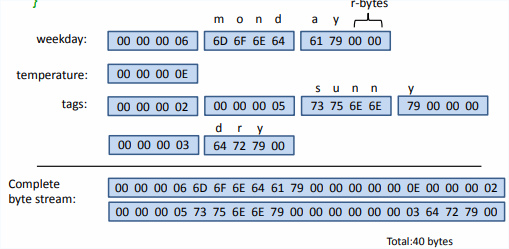
\includegraphics[width=.8\linewidth]{chap2_2.png} 
\lstinline{struct forecast:String weekday;int temperature;String tags<>;}
\rtext{ASN.1}:Abstract description of data types,telecommunication,internet protocol 
\textbar Enables exchange in heterogeneous systems
\textbar \btext{abstractSyntax $\overset{compiler}{\rightarrow}$ concreteSyntax Java, C++, they transfer syntax using encodingRules}
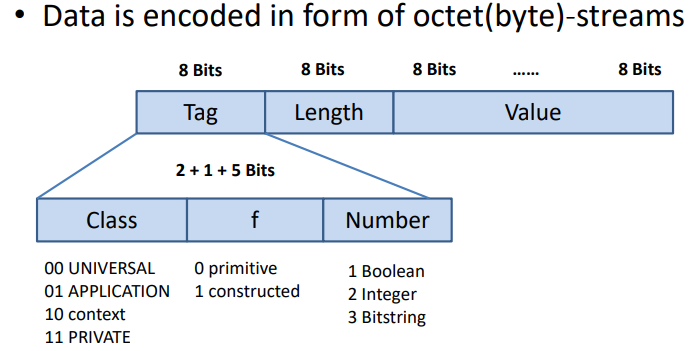
\includegraphics[width=.45\linewidth]{chap2_3.png}
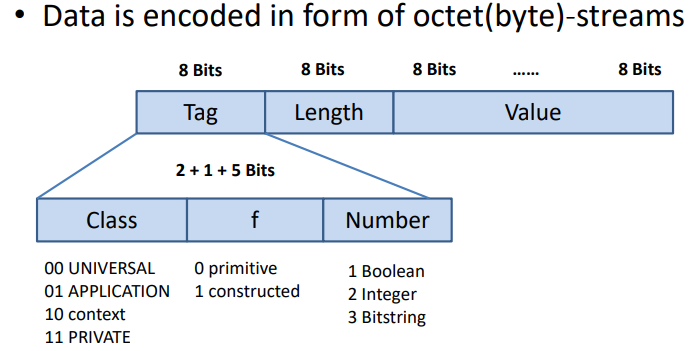
\includegraphics[width=.45\linewidth]{chap2_4.png}
\lstinline{Forecast::==SET{weekday IA5String,temperature Interger,tags SEQUENCE OF IS5String;}
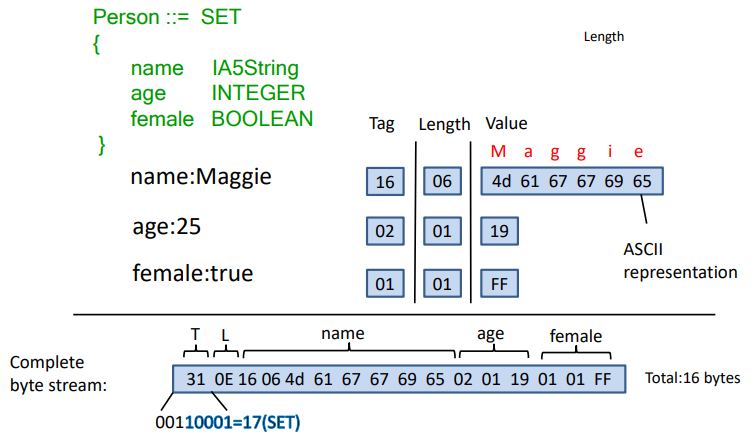
\includegraphics[width=.45\linewidth]{chap2_5.png}
\textbar encodes type information, +:receiver not need to know data description,-:additional overhead
\rtext{Java object serialization,JOS}
Stream-based transmission of serialized objects(Via TCP or UDP sockets)
, Receiver of object needs implementation of class
, Serialization does not require class specific code(Java reflection)
, Class implements java.io.Serializable interface
\textbf{-}: locked into Java(No support for heterogeneous systems), No support for versioning(If the serialized class changes, all network nodes
have to be updated)
\rtext{serialize:obj2bit}\lstinline{Socket s = new Socket("localhost", 8022);ObjectOutputStream oos = new ObjectOutputStream(s.getOutputStream()); oos.writeObject(obj);}
\rtext{deserialize:bit2obj}\lstinline{ServerSocket ss = new ServerSocket(8022);Socket s = serverSocket.accept();ObjectInputStream ois = new ObjectInputStream(s.getInputStream());obj=(Obj)ois.readObject();}
\rtext{XML}De facto standard for data exchange
\textbar Schema: \lstinline{<xsd:element name="forecast"> <xsd:complexType> <xsd:all> <xsd:element name="weekday" type="xsd:string"/> <xsd:element name="temperature" type="xsd:integer"/> <xsd:element name="tags">
<xsd:complexType> <xsd:sequence> <xsd:element name="tag" type="xsd:string" maxOccurs=\"unbounded\"/> </xsd:...>}
\textbar \lstinline{<forecast> <weekday>monday</weekday> <temperature>14</temperature> <tags> <tag>sunny</tag> <tag>dry</tag> </..>}
\rtext{JSON} human-readable text to transmit data objects
\textbar \lstinline{{"forecast":{"weekday":"monday","temperature" :14,"tags":["sunny","dry"] }\}\}}
\textbar \textbf{+ XML/JSON}:readable, defined as standard, JS support JSON(directly loaded  Browser and deserialized)
\textbar \textbf{- XML/JSON}: verbose, badPreformance, longOverhead, slowWriteParse
\rtext{ProtocolBuffersGoogle}: Similar concept like ASN.1, but not standard, efficient binary serialization, heterogeneous systems
\btext{data structures defined in .proto file(IDL) generate serialization code(Java, C$\#$), then java, .NET projects request, response each other}
\textbar .proto: \lstinline{message forecast{required string weekday =1 required int32 temperature =2 repeated string tags =3 }\}}
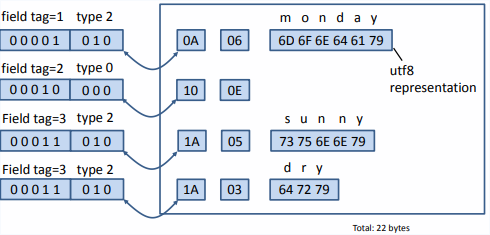
\includegraphics[width=.45\linewidth]{chap2_6.png}
\textbar \textbf{+:}efficient writing/parsing,well documented,Versioning \textbf{-:}No RPC
\rtext{ApacheThrift:framwork, applied Hadoop and HBase}
.thrift: \lstinline{struct Forecast{1: string weekday 2: i32 temperature 3: list<string> tags}\}}
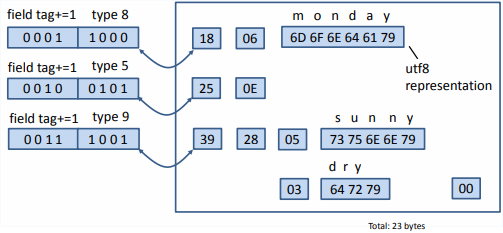
\includegraphics[width=.45\linewidth]{chap2_7.png}
\textbar \textbf{+:}Multiple protocols to serve different purposes(binary, JSON),RPC,Open source,widely,Versioning
\rtext{VariableLength:}
\end{multicols*}
\end{document}